% Options for packages loaded elsewhere
\PassOptionsToPackage{unicode}{hyperref}
\PassOptionsToPackage{hyphens}{url}
%
\documentclass[
]{book}
\usepackage{amsmath,amssymb}
\usepackage{lmodern}
\usepackage{ifxetex,ifluatex}
\ifnum 0\ifxetex 1\fi\ifluatex 1\fi=0 % if pdftex
  \usepackage[T1]{fontenc}
  \usepackage[utf8]{inputenc}
  \usepackage{textcomp} % provide euro and other symbols
\else % if luatex or xetex
  \usepackage{unicode-math}
  \defaultfontfeatures{Scale=MatchLowercase}
  \defaultfontfeatures[\rmfamily]{Ligatures=TeX,Scale=1}
\fi
% Use upquote if available, for straight quotes in verbatim environments
\IfFileExists{upquote.sty}{\usepackage{upquote}}{}
\IfFileExists{microtype.sty}{% use microtype if available
  \usepackage[]{microtype}
  \UseMicrotypeSet[protrusion]{basicmath} % disable protrusion for tt fonts
}{}
\makeatletter
\@ifundefined{KOMAClassName}{% if non-KOMA class
  \IfFileExists{parskip.sty}{%
    \usepackage{parskip}
  }{% else
    \setlength{\parindent}{0pt}
    \setlength{\parskip}{6pt plus 2pt minus 1pt}}
}{% if KOMA class
  \KOMAoptions{parskip=half}}
\makeatother
\usepackage{xcolor}
\IfFileExists{xurl.sty}{\usepackage{xurl}}{} % add URL line breaks if available
\IfFileExists{bookmark.sty}{\usepackage{bookmark}}{\usepackage{hyperref}}
\hypersetup{
  pdftitle={Technical Indicator Assembly Document for NOAA NaMES},
  pdfauthor={Willem Klajbor, The NOAA Ecosystem Indicators Working Group},
  hidelinks,
  pdfcreator={LaTeX via pandoc}}
\urlstyle{same} % disable monospaced font for URLs
\usepackage{color}
\usepackage{fancyvrb}
\newcommand{\VerbBar}{|}
\newcommand{\VERB}{\Verb[commandchars=\\\{\}]}
\DefineVerbatimEnvironment{Highlighting}{Verbatim}{commandchars=\\\{\}}
% Add ',fontsize=\small' for more characters per line
\usepackage{framed}
\definecolor{shadecolor}{RGB}{248,248,248}
\newenvironment{Shaded}{\begin{snugshade}}{\end{snugshade}}
\newcommand{\AlertTok}[1]{\textcolor[rgb]{0.94,0.16,0.16}{#1}}
\newcommand{\AnnotationTok}[1]{\textcolor[rgb]{0.56,0.35,0.01}{\textbf{\textit{#1}}}}
\newcommand{\AttributeTok}[1]{\textcolor[rgb]{0.77,0.63,0.00}{#1}}
\newcommand{\BaseNTok}[1]{\textcolor[rgb]{0.00,0.00,0.81}{#1}}
\newcommand{\BuiltInTok}[1]{#1}
\newcommand{\CharTok}[1]{\textcolor[rgb]{0.31,0.60,0.02}{#1}}
\newcommand{\CommentTok}[1]{\textcolor[rgb]{0.56,0.35,0.01}{\textit{#1}}}
\newcommand{\CommentVarTok}[1]{\textcolor[rgb]{0.56,0.35,0.01}{\textbf{\textit{#1}}}}
\newcommand{\ConstantTok}[1]{\textcolor[rgb]{0.00,0.00,0.00}{#1}}
\newcommand{\ControlFlowTok}[1]{\textcolor[rgb]{0.13,0.29,0.53}{\textbf{#1}}}
\newcommand{\DataTypeTok}[1]{\textcolor[rgb]{0.13,0.29,0.53}{#1}}
\newcommand{\DecValTok}[1]{\textcolor[rgb]{0.00,0.00,0.81}{#1}}
\newcommand{\DocumentationTok}[1]{\textcolor[rgb]{0.56,0.35,0.01}{\textbf{\textit{#1}}}}
\newcommand{\ErrorTok}[1]{\textcolor[rgb]{0.64,0.00,0.00}{\textbf{#1}}}
\newcommand{\ExtensionTok}[1]{#1}
\newcommand{\FloatTok}[1]{\textcolor[rgb]{0.00,0.00,0.81}{#1}}
\newcommand{\FunctionTok}[1]{\textcolor[rgb]{0.00,0.00,0.00}{#1}}
\newcommand{\ImportTok}[1]{#1}
\newcommand{\InformationTok}[1]{\textcolor[rgb]{0.56,0.35,0.01}{\textbf{\textit{#1}}}}
\newcommand{\KeywordTok}[1]{\textcolor[rgb]{0.13,0.29,0.53}{\textbf{#1}}}
\newcommand{\NormalTok}[1]{#1}
\newcommand{\OperatorTok}[1]{\textcolor[rgb]{0.81,0.36,0.00}{\textbf{#1}}}
\newcommand{\OtherTok}[1]{\textcolor[rgb]{0.56,0.35,0.01}{#1}}
\newcommand{\PreprocessorTok}[1]{\textcolor[rgb]{0.56,0.35,0.01}{\textit{#1}}}
\newcommand{\RegionMarkerTok}[1]{#1}
\newcommand{\SpecialCharTok}[1]{\textcolor[rgb]{0.00,0.00,0.00}{#1}}
\newcommand{\SpecialStringTok}[1]{\textcolor[rgb]{0.31,0.60,0.02}{#1}}
\newcommand{\StringTok}[1]{\textcolor[rgb]{0.31,0.60,0.02}{#1}}
\newcommand{\VariableTok}[1]{\textcolor[rgb]{0.00,0.00,0.00}{#1}}
\newcommand{\VerbatimStringTok}[1]{\textcolor[rgb]{0.31,0.60,0.02}{#1}}
\newcommand{\WarningTok}[1]{\textcolor[rgb]{0.56,0.35,0.01}{\textbf{\textit{#1}}}}
\usepackage{longtable,booktabs,array}
\usepackage{calc} % for calculating minipage widths
% Correct order of tables after \paragraph or \subparagraph
\usepackage{etoolbox}
\makeatletter
\patchcmd\longtable{\par}{\if@noskipsec\mbox{}\fi\par}{}{}
\makeatother
% Allow footnotes in longtable head/foot
\IfFileExists{footnotehyper.sty}{\usepackage{footnotehyper}}{\usepackage{footnote}}
\makesavenoteenv{longtable}
\usepackage{graphicx}
\makeatletter
\def\maxwidth{\ifdim\Gin@nat@width>\linewidth\linewidth\else\Gin@nat@width\fi}
\def\maxheight{\ifdim\Gin@nat@height>\textheight\textheight\else\Gin@nat@height\fi}
\makeatother
% Scale images if necessary, so that they will not overflow the page
% margins by default, and it is still possible to overwrite the defaults
% using explicit options in \includegraphics[width, height, ...]{}
\setkeys{Gin}{width=\maxwidth,height=\maxheight,keepaspectratio}
% Set default figure placement to htbp
\makeatletter
\def\fps@figure{htbp}
\makeatother
\setlength{\emergencystretch}{3em} % prevent overfull lines
\providecommand{\tightlist}{%
  \setlength{\itemsep}{0pt}\setlength{\parskip}{0pt}}
\setcounter{secnumdepth}{5}
\usepackage{booktabs}
\usepackage{amsthm}
\makeatletter
\def\thm@space@setup{%
  \thm@preskip=8pt plus 2pt minus 4pt
  \thm@postskip=\thm@preskip
}
\makeatother
\ifluatex
  \usepackage{selnolig}  % disable illegal ligatures
\fi
\usepackage[]{natbib}
\bibliographystyle{apalike}

\title{Technical Indicator Assembly Document for NOAA NaMES}
\author{Willem Klajbor, The NOAA Ecosystem Indicators Working Group}
\date{2021-07-08}

\begin{document}
\maketitle

{
\setcounter{tocdepth}{1}
\tableofcontents
}
\hypertarget{overview}{%
\chapter*{Overview}\label{overview}}
\addcontentsline{toc}{chapter}{Overview}

The National Marine Ecosystem Status web portal provides the status of marine ecosystems across the U.S. and access to NOAA ecosystem indicator information and data. This website is designed to document the data sources and methods used to create the indicators displayed on the site.

\hypertarget{definition-of-indicators}{%
\section{Definition of Indicators}\label{definition-of-indicators}}

Ecosystem indicators are quantitative and/or qualitative measures of key components of the ecosystem. Marine ecosystems provide food, jobs, security, well-being, and other services to millions of people across the U.S. Yet, marine ecosystems and the people that rely on them are facing increasingly complex challenges. Tracking the status and trends of ocean and coastal ecosystems is critically important to understand how these ecosystems are changing and identify potential issues.

\hypertarget{chlorophyll-a}{%
\chapter{Chlorophyll-a}\label{chlorophyll-a}}

\hypertarget{data}{%
\section{Data}\label{data}}

Under Construction

\hypertarget{methods}{%
\section{Methods}\label{methods}}

Under construction

\hypertarget{zooplankton}{%
\chapter{Zooplankton}\label{zooplankton}}

\hypertarget{data-1}{%
\section{Data}\label{data-1}}

Under Construction

\hypertarget{methods-1}{%
\section{Methods}\label{methods-1}}

Under construction

\hypertarget{coral-reefs}{%
\chapter{Coral Reefs}\label{coral-reefs}}

\hypertarget{data-2}{%
\section{Data}\label{data-2}}

Under Construction

\hypertarget{methods-2}{%
\section{Methods}\label{methods-2}}

Under construction

\hypertarget{forage-fish}{%
\chapter{Forage Fish}\label{forage-fish}}

\hypertarget{data-3}{%
\section{Data}\label{data-3}}

Under Construction

\hypertarget{methods-3}{%
\section{Methods}\label{methods-3}}

Under construction

\hypertarget{seabirds}{%
\chapter{Seabirds}\label{seabirds}}

\hypertarget{data-4}{%
\section{Data}\label{data-4}}

Under Construction

\hypertarget{methods-4}{%
\section{Methods}\label{methods-4}}

Under construction

\hypertarget{overfished-stocks}{%
\chapter{Overfished Stocks}\label{overfished-stocks}}

Fish play an important role in marine ecosystems, supporting the ecological structure of many marine food webs. Caught by recreational and commercial fisheries, fish support significant parts of coastal economies, and can play an important cultural role in many regions. To understand the health of fish populations - as well as their abundance and distribution, we regularly assess fish stocks - stock assessments. Assessments let us know if a stock is experiencing overfishing or if it is overfished i.e.~how much catch is sustainable while maintaining a healthy stock. And, if a stock becomes depleted, stock assessments can help determine what steps may be taken to rebuild it to sustainable levels. Understanding stock assessments helps measure how well we're managing and recovering fish stocks over time.

We present the number of overfished stocks by year in all regions.

\hypertarget{data-5}{%
\section{Data}\label{data-5}}

Data are obtained from the NOAA Fisheries Fishery Stock Status website \url{https://www.fisheries.noaa.gov/national/population-assessments/fishery-stock-status-updates}. Stocks that meet the criteria for overfished status are summed by year for each region. The status of stocks are available in report form and graphically.

\hypertarget{methods-5}{%
\section{Methods}\label{methods-5}}

This indicator is compiled manually.

After traveling to \url{https://www.fisheries.noaa.gov/national/population-assessments/fishery-stock-status-updates}, identify the most up to date status report. The reports should be available in two formats - through a report and through a visual.

The easiest way to compile the data are using the visual, which should be named ``Stocks on the Overfished and Overfishing Lists by Region.'' After opening the visual (example below), overfished stocks will be displayed by sqaures and sorted spatially by region. We are only counting the ``Overfished'' stocks - do not count stocks that are only on the ``Overfishing'' list.

\begin{Shaded}
\begin{Highlighting}[]
\NormalTok{knitr}\SpecialCharTok{::}\FunctionTok{include\_graphics}\NormalTok{(}\FunctionTok{rep}\NormalTok{(}\StringTok{"overfished.png"}\NormalTok{))}
\end{Highlighting}
\end{Shaded}

\begin{figure}
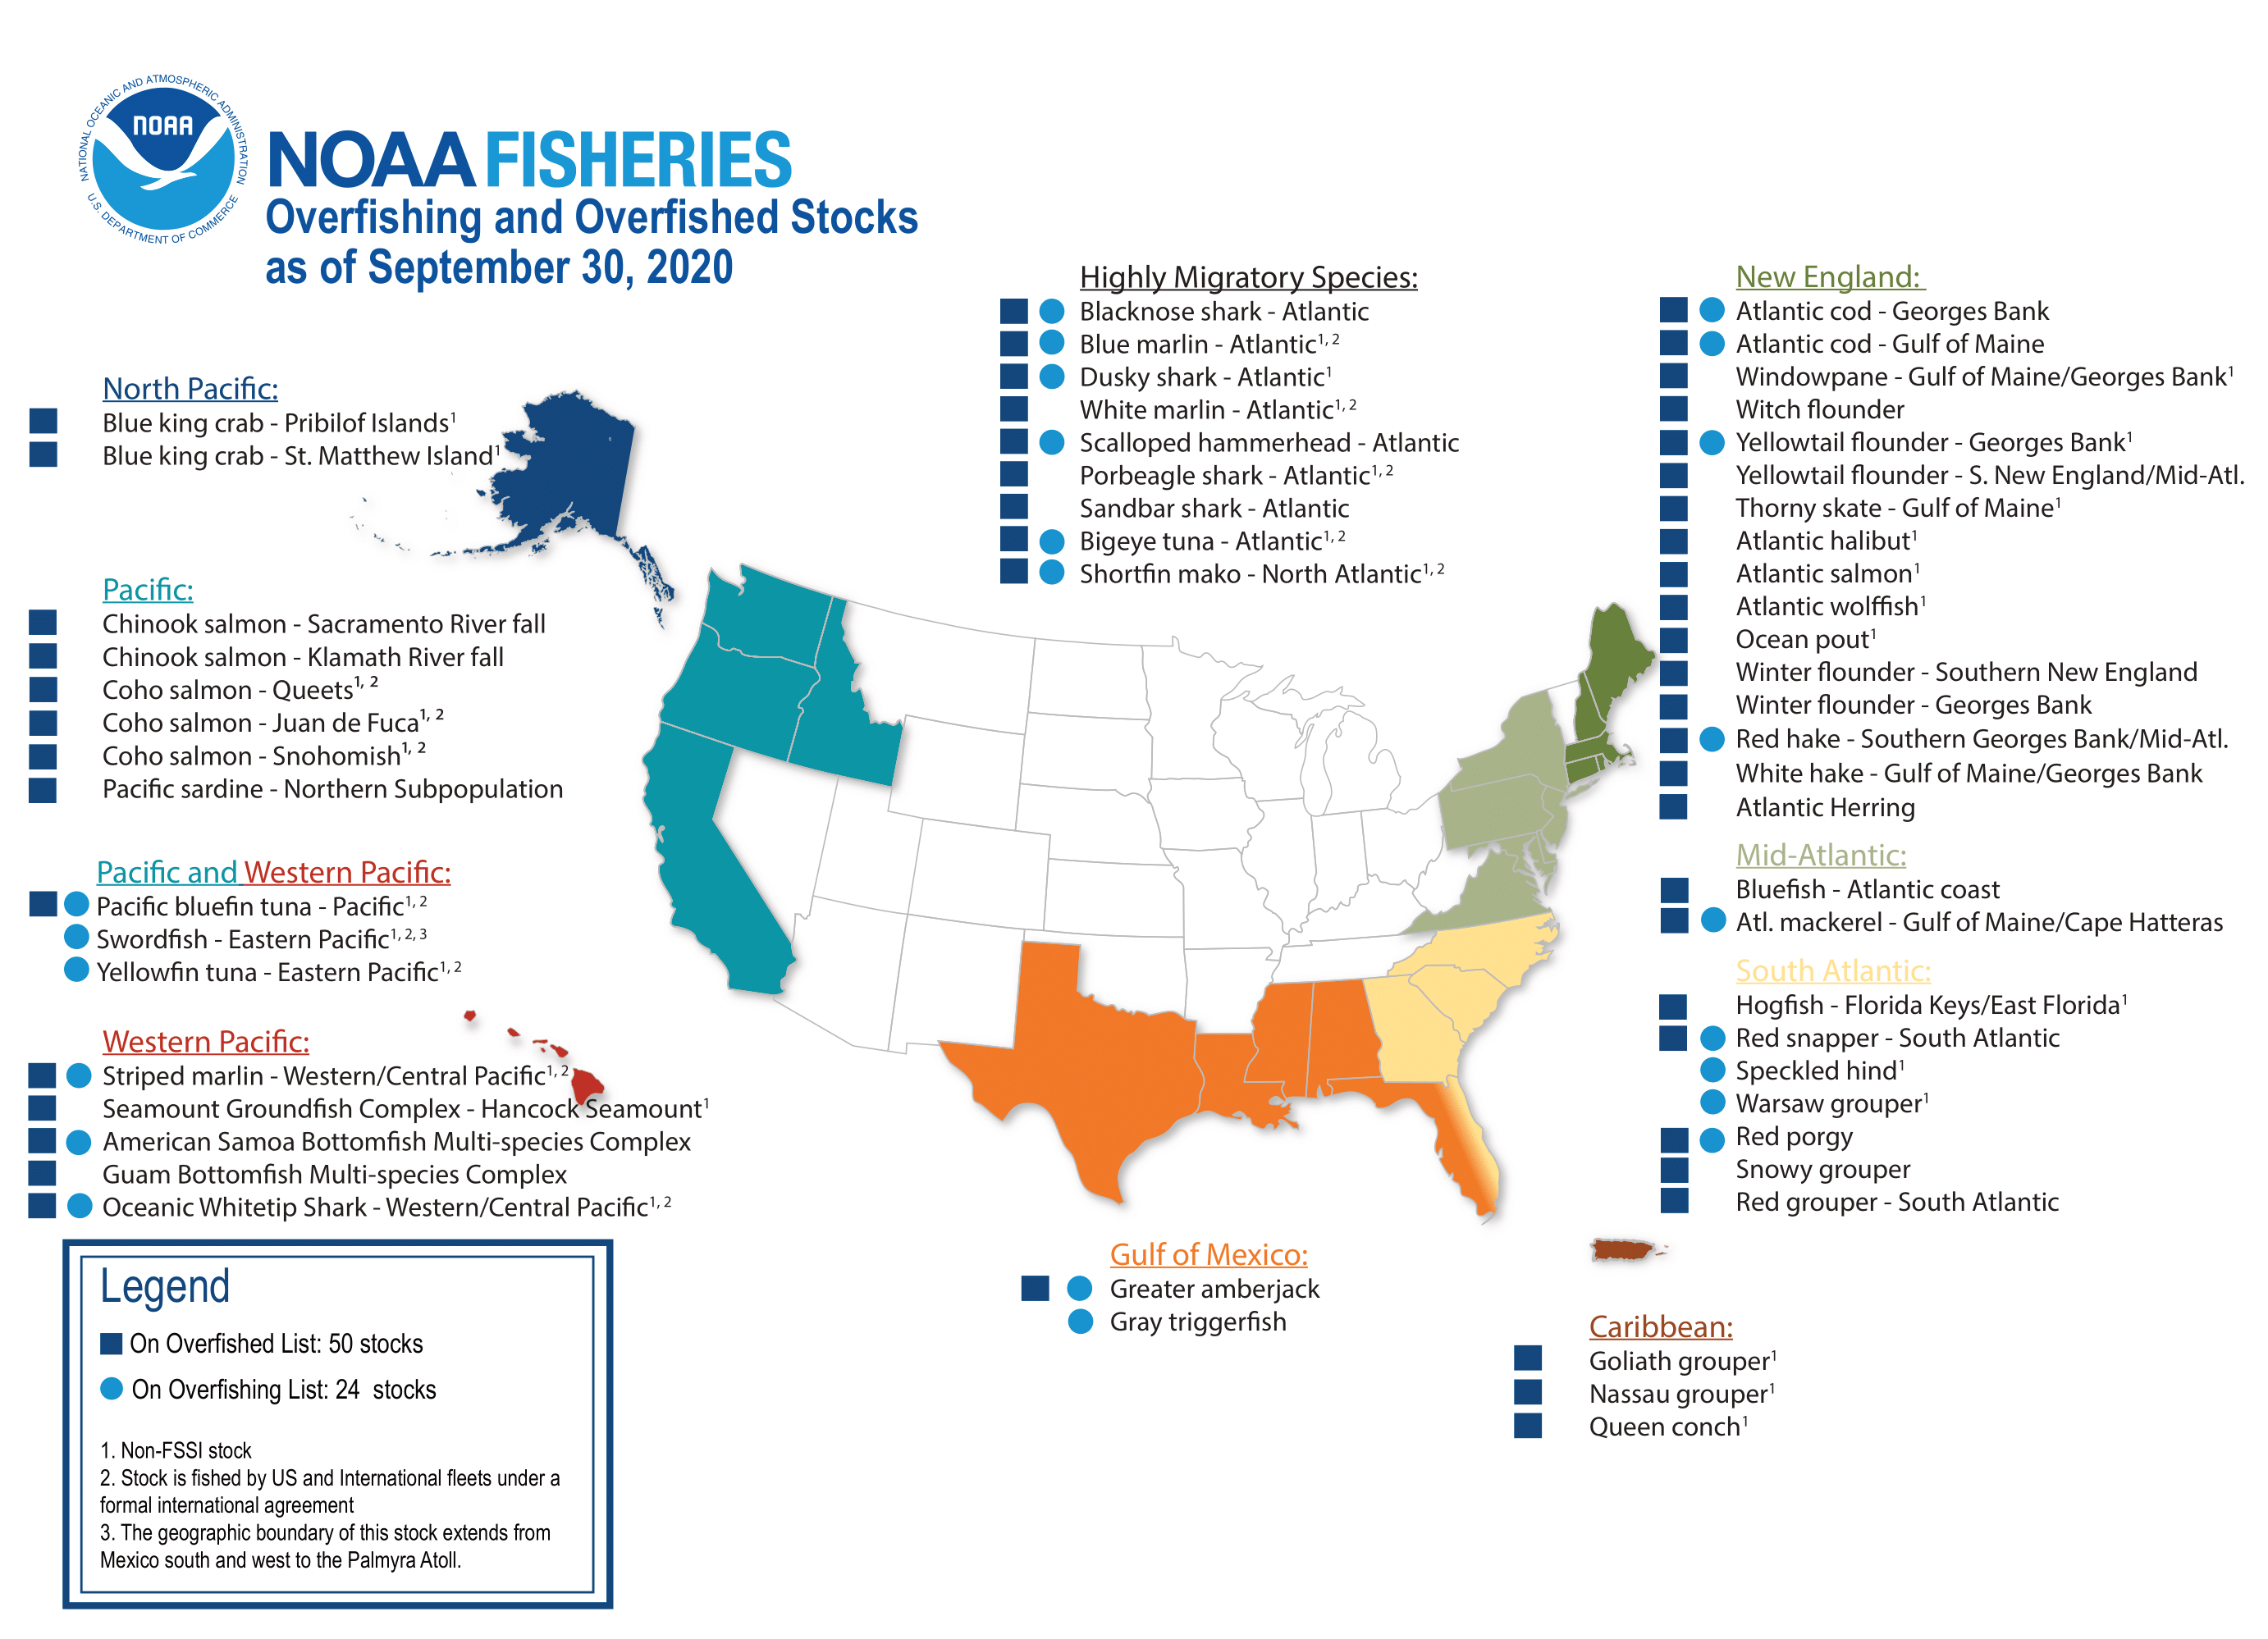
\includegraphics[width=38.39in]{overfished} \caption{NOAA Fisheries 2020 Q4 Stock Status Map}\label{fig:unnamed-chunk-2}
\end{figure}

North Pacific corresponds to the Alaska Region, Pacific corresponds to the California Current, Western Pacific corresponds to Hawaii (but be sure not to count the pacific island specific complexes), and New England corresponds to North Atlantic.

For more information, contact Willem Klajbor (\href{mailto:willem.klajbor@noaa.gov}{\nolinkurl{willem.klajbor@noaa.gov}}) or Stephanie Oakes (\href{mailto:stephanie.oakes@noaa.gov}{\nolinkurl{stephanie.oakes@noaa.gov}}).

\hypertarget{marine-mammals}{%
\chapter{Marine Mammals}\label{marine-mammals}}

\hypertarget{esa}{%
\section{ESA}\label{esa}}

\hypertarget{data-6}{%
\subsection{Data}\label{data-6}}

Under Construction

\hypertarget{methods-6}{%
\subsection{Methods}\label{methods-6}}

Under construction

\hypertarget{mmpa}{%
\section{MMPA}\label{mmpa}}

\hypertarget{data-7}{%
\subsection{Data}\label{data-7}}

Under Construction

\hypertarget{methods-7}{%
\subsection{Methods}\label{methods-7}}

Under construction

\hypertarget{unusual-mortality-events}{%
\chapter{Unusual Mortality Events}\label{unusual-mortality-events}}

\hypertarget{data-8}{%
\section{Data}\label{data-8}}

Under Construction

\hypertarget{methods-8}{%
\section{Methods}\label{methods-8}}

Under construction

\hypertarget{sea-surface-temperature}{%
\chapter{Sea Surface Temperature}\label{sea-surface-temperature}}

\hypertarget{data-9}{%
\section{Data}\label{data-9}}

Under Construction

\hypertarget{methods-9}{%
\section{Methods}\label{methods-9}}

Under construction

\hypertarget{sea-level}{%
\chapter{Sea Level}\label{sea-level}}

\hypertarget{data-10}{%
\section{Data}\label{data-10}}

Under Construction

\hypertarget{methods-10}{%
\section{Methods}\label{methods-10}}

Under construction

\hypertarget{sea-ice}{%
\chapter{Sea Ice}\label{sea-ice}}

Unlike icebergs, glaciers, ice sheets, and ice shelves, which originate on land, sea ice forms, expands, and melts in the ocean. Sea ice influences global climate by reflecting sunlight back into space. Because this solar energy is not absorbed into the ocean, temperatures nearer the poles remain cool. When sea ice melts, the surface area reflecting sunlight decreases, allowing more solar energy to be absorbed by the ocean, causing temperatures to rise. This creates a positive feedback loop. Warmer water temperatures delay ice growth in the autumn and winter, and the ice melts faster the following spring, exposing dark ocean waters for longer periods the following summer.

Sea ice affects the movement of ocean waters. When sea ice forms, ocean salts are left behind. As the seawater gets saltier, its density increases, and it sinks. Surface water is pulled in to replace the sinking water, which in turn becomes cold and salty and sinks. This initiates deep-ocean currents driving the global ocean conveyor belt.

Sea ice is an important element of the Arctic system. It provides an important habitat for biological activity, i.e.~algae grows on the bottom of sea ice, forming the basis of the Arctic food web, and it plays a critical role in the life cycle of many marine mammals - seals and polar bears. Sea ice also serves a critical role in supporting Indigenous communities culture and survival. We present the annual sea ice extent in millions of Kilometers for the Arctic region.

\hypertarget{data-11}{%
\section{Data}\label{data-11}}

Sea ice data was accessed from the NOAA National Centers for Environmental Information, \url{https://www.ncdc.noaa.gov/snow-and-ice/extent/} , with the data pulled from here: \url{https://www.ncdc.noaa.gov/snow-and-ice/extent/sea-ice/N/3/data.csv}. The data are plotted in units of million square km.

\hypertarget{methods-11}{%
\section{Methods}\label{methods-11}}

To download the current sea ice data, you can either:

\begin{enumerate}
\def\labelenumi{\arabic{enumi})}
\tightlist
\item
  Copy/paste the following url into your web browser:
  \url{https://www.ncdc.noaa.gov/snow-and-ice/extent/sea-ice/N/3/data.csv}
\end{enumerate}

or

\begin{enumerate}
\def\labelenumi{\arabic{enumi})}
\setcounter{enumi}{1}
\tightlist
\item
  Use the following R code to download the data and import it into your RStudio environment
\end{enumerate}

\begin{Shaded}
\begin{Highlighting}[]
\NormalTok{url }\OtherTok{\textless{}{-}}\StringTok{"https://www.ncdc.noaa.gov/snow{-}and{-}ice/extent/sea{-}ice/N/3/data.csv"}
\CommentTok{\# Specify destination where file should be saved}
\NormalTok{destfile }\OtherTok{\textless{}{-}} \StringTok{"C:/Users/ ... Your Path ... /my folder/output.csv"}
\CommentTok{\#Apply download.file function in R}
\FunctionTok{download.file}\NormalTok{(url, destfile)}
\end{Highlighting}
\end{Shaded}

Data were restructured and gauge values were calculated manually.

For more information, contact Willem Klajbor (\href{mailto:willem.klajbor@noaa.gov}{\nolinkurl{willem.klajbor@noaa.gov}}) or Scott Cross (\href{mailto:scott.cross@noaa.gov}{\nolinkurl{scott.cross@noaa.gov}}).

\hypertarget{climate-indices}{%
\chapter{Climate Indices}\label{climate-indices}}

\hypertarget{enso}{%
\section{ENSO}\label{enso}}

Under Construction

\hypertarget{mei}{%
\section{MEI}\label{mei}}

Under construction

\hypertarget{pdo}{%
\section{PDO}\label{pdo}}

Under Construction

\hypertarget{epnp}{%
\section{EPNP}\label{epnp}}

Under Construction

\hypertarget{nao}{%
\section{NAO}\label{nao}}

Under Construction

\hypertarget{amo}{%
\section{AMO}\label{amo}}

Under Construction

\hypertarget{coastal-population}{%
\chapter{Coastal Population}\label{coastal-population}}

\hypertarget{data-12}{%
\section{Data}\label{data-12}}

Under Construction

\hypertarget{methods-12}{%
\section{Methods}\label{methods-12}}

Under construction

\hypertarget{coastal-tourism}{%
\chapter{Coastal Tourism}\label{coastal-tourism}}

\hypertarget{data-13}{%
\section{Data}\label{data-13}}

Under Construction

\hypertarget{methods-13}{%
\section{Methods}\label{methods-13}}

Under construction

\hypertarget{coastal-employment}{%
\chapter{Coastal Employment}\label{coastal-employment}}

\hypertarget{data-14}{%
\section{Data}\label{data-14}}

Under Construction

\hypertarget{methods-14}{%
\section{Methods}\label{methods-14}}

Under construction

\hypertarget{commercial-fishing}{%
\chapter{Commercial Fishing}\label{commercial-fishing}}

\hypertarget{landings}{%
\section{Landings}\label{landings}}

\hypertarget{data-15}{%
\subsection{Data}\label{data-15}}

Under Construction

\hypertarget{methods-15}{%
\subsection{Methods}\label{methods-15}}

Under construction

\hypertarget{revenue}{%
\section{Revenue}\label{revenue}}

\hypertarget{data-16}{%
\subsection{Data}\label{data-16}}

Under Construction

\hypertarget{methods-16}{%
\subsection{Methods}\label{methods-16}}

Under construction

\hypertarget{recreational-fishing}{%
\chapter{Recreational Fishing}\label{recreational-fishing}}

\hypertarget{effort}{%
\section{Effort}\label{effort}}

\hypertarget{data-17}{%
\subsection{Data}\label{data-17}}

Under Construction

\hypertarget{methods-17}{%
\subsection{Methods}\label{methods-17}}

Under construction

\hypertarget{harvest}{%
\section{Harvest}\label{harvest}}

\hypertarget{data-18}{%
\subsection{Data}\label{data-18}}

Under Construction

\hypertarget{methods-18}{%
\subsection{Methods}\label{methods-18}}

Under construction

\hypertarget{fishing-engagement}{%
\chapter{Fishing Engagement}\label{fishing-engagement}}

\hypertarget{commercial}{%
\section{Commercial}\label{commercial}}

\hypertarget{data-19}{%
\subsection{Data}\label{data-19}}

Under Construction

\hypertarget{methods-19}{%
\subsection{Methods}\label{methods-19}}

Under construction

\hypertarget{recreational}{%
\section{Recreational}\label{recreational}}

\hypertarget{data-20}{%
\subsection{Data}\label{data-20}}

Under Construction

\hypertarget{methods-20}{%
\subsection{Methods}\label{methods-20}}

Under construction

\hypertarget{billion-dollar-disasters}{%
\chapter{Billion Dollar Disasters}\label{billion-dollar-disasters}}

In the United States the number of weather and climate-related disasters exceeding 1 billion dollars has been increasing since 1980. These events have significant impacts to coastal economies and communities. The Billion Dollar Disaster indicator provides information on the frequency and the total estimated costs of major weather and climate events that occur in the United States. This indicator compiles the annual number of weather and climate-related disasters across seven event types. Events are included if they are estimated to cause more than one billion U.S. dollars in direct losses. The cost estimates of these events are adjusted for inflation using the Consumer Price Index (CPI) and are based on costs documented in several Federal and private-sector databases. We present the total annual number of disaster events for all regions.

\hypertarget{data-21}{%
\section{Data}\label{data-21}}

Billion dollar disaster event frequency data are taken from NOAA's National Centers for Environmental Information (\url{https://www.ncdc.noaa.gov/billions/}). The number of disasters within each region were summed for every year of available data. Although the number is the count of unique disaster events within a region, the same disaster can impact multiple regions, meaning a sum across regions will overestimate the unique number of disasters.

\hypertarget{methods-need-qc}{%
\section{Methods (need QC)}\label{methods-need-qc}}

The Billion Dollar Event Frequency Data displayed on the website were compiled using the following code:

\begin{Shaded}
\begin{Highlighting}[]
\NormalTok{PKG }\OtherTok{\textless{}{-}} \FunctionTok{c}\NormalTok{(}\StringTok{"foreign"}\NormalTok{,}\StringTok{"stringr"}\NormalTok{,}\StringTok{"data.table"}\NormalTok{)}

\ControlFlowTok{for}\NormalTok{ (p }\ControlFlowTok{in}\NormalTok{ PKG) \{}
  \ControlFlowTok{if}\NormalTok{(}\SpecialCharTok{!}\FunctionTok{require}\NormalTok{(p,}\AttributeTok{character.only =} \ConstantTok{TRUE}\NormalTok{)) \{  }
    \FunctionTok{install.packages}\NormalTok{(p)}
    \FunctionTok{require}\NormalTok{(p,}\AttributeTok{character.only =} \ConstantTok{TRUE}\NormalTok{)\}}
\NormalTok{\}}

\CommentTok{\#states \textless{}{-} c("AK","AL","AR","AZ","CA","CO","CT","DE","FL","GA","HI",}
\CommentTok{\#            "IA","ID","IL","IN","KS","KY","LA","MA","MD","ME","MI",}
\CommentTok{\#            "MN","MO","MS","MT","NC","ND","NE","NH","NJ","NM","NV",}
\CommentTok{\#            "NY","OH","OK","OR","PA","RI","SC","SD","TN","TX","UT",}
\CommentTok{\#           "VA","VT","WA","WI","WV","WY")}

\NormalTok{states }\OtherTok{\textless{}{-}} \FunctionTok{c}\NormalTok{(}\StringTok{"AK"}\NormalTok{,}\StringTok{"AL"}\NormalTok{,}\StringTok{"CA"}\NormalTok{,}\StringTok{"CT"}\NormalTok{,}\StringTok{"DE"}\NormalTok{,}\StringTok{"FL"}\NormalTok{,}\StringTok{"GA"}\NormalTok{,}\StringTok{"HI"}\NormalTok{,}
            \StringTok{"LA"}\NormalTok{,}\StringTok{"MA"}\NormalTok{,}\StringTok{"MD"}\NormalTok{,}\StringTok{"ME"}\NormalTok{,}
            \StringTok{"MS"}\NormalTok{,}\StringTok{"NC"}\NormalTok{,}\StringTok{"NH"}\NormalTok{,}\StringTok{"NJ"}\NormalTok{,}
            \StringTok{"NY"}\NormalTok{,}\StringTok{"OR"}\NormalTok{,}\StringTok{"PA"}\NormalTok{,}\StringTok{"RI"}\NormalTok{,}\StringTok{"SC"}\NormalTok{,}\StringTok{"TX"}\NormalTok{,}
            \StringTok{"VA"}\NormalTok{,}\StringTok{"WA"}\NormalTok{,}\StringTok{"PR"}\NormalTok{,}\StringTok{"VI"}\NormalTok{)}

\CommentTok{\#Update Year in URL (2021)}
\NormalTok{Billion\_Storm }\OtherTok{\textless{}{-}} \ConstantTok{NULL}
\ControlFlowTok{for}\NormalTok{ (x }\ControlFlowTok{in}\NormalTok{ states) \{}
\NormalTok{  temp }\OtherTok{\textless{}{-}} \FunctionTok{tempfile}\NormalTok{()}
\NormalTok{  temp.connect }\OtherTok{\textless{}{-}} \FunctionTok{url}\NormalTok{(}\FunctionTok{paste0}\NormalTok{(}\StringTok{"https://www.ncdc.noaa.gov/billions/events{-}"}\NormalTok{,x,}\StringTok{"{-}1980{-}2021.csv"}\NormalTok{, }\AttributeTok{sep=}\StringTok{""}\NormalTok{))}
\NormalTok{  temp }\OtherTok{\textless{}{-}} \FunctionTok{data.table}\NormalTok{(}\FunctionTok{read.delim}\NormalTok{(temp.connect, }\AttributeTok{header=}\ConstantTok{TRUE}\NormalTok{,}\AttributeTok{fill=}\ConstantTok{FALSE}\NormalTok{, }\AttributeTok{stringsAsFactors=}\ConstantTok{FALSE}\NormalTok{,}\AttributeTok{skip=}\DecValTok{1}\NormalTok{, }\AttributeTok{sep=}\StringTok{","}\NormalTok{))}
\NormalTok{  temp}\SpecialCharTok{$}\NormalTok{State }\OtherTok{\textless{}{-}}\NormalTok{ x}
\NormalTok{  Billion\_Storm }\OtherTok{\textless{}{-}} \FunctionTok{rbind}\NormalTok{(Billion\_Storm,temp)}
  \FunctionTok{unlink}\NormalTok{(temp)}
  \FunctionTok{rm}\NormalTok{(temp)}
\NormalTok{\}}

\NormalTok{Billion\_Storm}\SpecialCharTok{$}\NormalTok{Begin.Date }\OtherTok{\textless{}{-}} \FunctionTok{as.character}\NormalTok{(Billion\_Storm}\SpecialCharTok{$}\NormalTok{Begin.Date)}
\NormalTok{Billion\_Storm}\SpecialCharTok{$}\NormalTok{Begin.Year }\OtherTok{\textless{}{-}}  \FunctionTok{substr}\NormalTok{(Billion\_Storm}\SpecialCharTok{$}\NormalTok{Begin.Date,}\DecValTok{1}\NormalTok{,}\DecValTok{4}\NormalTok{)}
\NormalTok{Billion\_Storm}\SpecialCharTok{$}\NormalTok{Begin.Date }\OtherTok{\textless{}{-}} \FunctionTok{as.Date}\NormalTok{(Billion\_Storm}\SpecialCharTok{$}\NormalTok{Begin.Date,}\StringTok{"\%Y \%m \%d"}\NormalTok{)}
\NormalTok{Billion\_Storm}\SpecialCharTok{$}\NormalTok{End.Date }\OtherTok{\textless{}{-}} \FunctionTok{as.character}\NormalTok{(Billion\_Storm}\SpecialCharTok{$}\NormalTok{End.Date)}
\NormalTok{Billion\_Storm}\SpecialCharTok{$}\NormalTok{End.Year }\OtherTok{\textless{}{-}}  \FunctionTok{substr}\NormalTok{(Billion\_Storm}\SpecialCharTok{$}\NormalTok{End.Date,}\DecValTok{1}\NormalTok{,}\DecValTok{4}\NormalTok{)}
\NormalTok{Billion\_Storm}\SpecialCharTok{$}\NormalTok{End.Date }\OtherTok{\textless{}{-}} \FunctionTok{as.Date}\NormalTok{(Billion\_Storm}\SpecialCharTok{$}\NormalTok{End.Date,}\StringTok{"\%Y \%m \%d"}\NormalTok{)}

\NormalTok{Gulf.of.Mexico }\OtherTok{\textless{}{-}} \FunctionTok{c}\NormalTok{(}\StringTok{"FL"}\NormalTok{,}\StringTok{"AL"}\NormalTok{,}\StringTok{"LA"}\NormalTok{,}\StringTok{"MS"}\NormalTok{,}\StringTok{"TX"}\NormalTok{)}
\NormalTok{Northeast }\OtherTok{\textless{}{-}} \FunctionTok{c}\NormalTok{(}\StringTok{"NC"}\NormalTok{,}\StringTok{"VA"}\NormalTok{,}\StringTok{"MD"}\NormalTok{,}\StringTok{"DE"}\NormalTok{,}\StringTok{"PA"}\NormalTok{,}\StringTok{"NJ"}\NormalTok{,}\StringTok{"NY"}\NormalTok{,}\StringTok{"CT"}\NormalTok{,}\StringTok{"RI"}\NormalTok{,}
               \StringTok{"MA"}\NormalTok{,}\StringTok{"NH"}\NormalTok{,}\StringTok{"ME"}\NormalTok{)}
\NormalTok{Southeast }\OtherTok{\textless{}{-}} \FunctionTok{c}\NormalTok{(}\StringTok{"SC"}\NormalTok{,}\StringTok{"GA"}\NormalTok{,}\StringTok{"FL"}\NormalTok{)}
\NormalTok{California.Current }\OtherTok{\textless{}{-}} \FunctionTok{c}\NormalTok{(}\StringTok{"CA"}\NormalTok{,}\StringTok{"OR"}\NormalTok{,}\StringTok{"WA"}\NormalTok{)}
\NormalTok{Alaska}\OtherTok{\textless{}{-}} \FunctionTok{c}\NormalTok{(}\StringTok{"AK"}\NormalTok{)}
\NormalTok{Hawaii }\OtherTok{\textless{}{-}} \FunctionTok{c}\NormalTok{(}\StringTok{"HI"}\NormalTok{)}
\NormalTok{Caribbean }\OtherTok{\textless{}{-}} \FunctionTok{c}\NormalTok{(}\StringTok{"PR"}\NormalTok{,}\StringTok{"VI"}\NormalTok{)}

\NormalTok{Storm\_Freq }\OtherTok{\textless{}{-}} \ConstantTok{NULL}
\ControlFlowTok{for}\NormalTok{ (x }\ControlFlowTok{in} \FunctionTok{c}\NormalTok{(}\StringTok{"Gulf.of.Mexico"}\NormalTok{,}\StringTok{"Northeast"}\NormalTok{,}\StringTok{"Southeast"}\NormalTok{,}\StringTok{"California.Current"}\NormalTok{,}\StringTok{"Alaska"}\NormalTok{,}\StringTok{"Hawaii"}\NormalTok{,}\StringTok{"Caribbean"}\NormalTok{)) \{}
\NormalTok{  TEMP }\OtherTok{\textless{}{-}}\NormalTok{ Billion\_Storm[}\FunctionTok{which}\NormalTok{(Billion\_Storm}\SpecialCharTok{$}\NormalTok{State}\SpecialCharTok{\%in\%}\FunctionTok{get}\NormalTok{(x)),]}
\NormalTok{  TEMP}\SpecialCharTok{$}\NormalTok{Disaster }\OtherTok{\textless{}{-}}\NormalTok{ TEMP}\SpecialCharTok{$}\NormalTok{Begin.Date }\OtherTok{\textless{}{-}}\NormalTok{ TEMP}\SpecialCharTok{$}\NormalTok{End.Date }\OtherTok{\textless{}{-}}\NormalTok{ TEMP}\SpecialCharTok{$}\NormalTok{Deaths }\OtherTok{\textless{}{-}}\NormalTok{ TEMP}\SpecialCharTok{$}\NormalTok{State }\OtherTok{\textless{}{-}}\NormalTok{ TEMP}\SpecialCharTok{$}\NormalTok{Begin.Year }\OtherTok{\textless{}{-}} \ConstantTok{NULL}
\NormalTok{  TEMP }\OtherTok{\textless{}{-}} \FunctionTok{unique}\NormalTok{(TEMP)}
  \FunctionTok{colnames}\NormalTok{(TEMP)}\OtherTok{\textless{}{-}} \FunctionTok{c}\NormalTok{(}\StringTok{\textquotesingle{}Name\textquotesingle{}}\NormalTok{,}\StringTok{\textquotesingle{}Frequency\textquotesingle{}}\NormalTok{,}\StringTok{\textquotesingle{}End.Year\textquotesingle{}}\NormalTok{)}
\NormalTok{  TEMP }\OtherTok{\textless{}{-}} \FunctionTok{aggregate}\NormalTok{(Frequency}\SpecialCharTok{\textasciitilde{}}\NormalTok{End.Year, }\AttributeTok{data=}\NormalTok{TEMP, }\AttributeTok{FUN=}\NormalTok{length)}
\NormalTok{  TEMP}\SpecialCharTok{$}\NormalTok{Region }\OtherTok{\textless{}{-}}\NormalTok{ x}
  \FunctionTok{assign}\NormalTok{(}\FunctionTok{paste0}\NormalTok{(x,}\StringTok{"\_Data"}\NormalTok{, }\AttributeTok{sep=}\StringTok{""}\NormalTok{),TEMP)}
\NormalTok{  Storm\_Freq }\OtherTok{\textless{}{-}} \FunctionTok{rbind}\NormalTok{(Storm\_Freq,TEMP)}
  \FunctionTok{rm}\NormalTok{(TEMP)}
\NormalTok{\}}

\NormalTok{Storm\_Freq\_F }\OtherTok{\textless{}{-}} \FunctionTok{spread}\NormalTok{(Storm\_Freq,Region,Frequency)}

\FunctionTok{write.csv}\NormalTok{(Storm\_Freq\_F,}\AttributeTok{file=}\StringTok{"C:/Users/... your path.../Billion\_Dollar\_Storms\_1980\_Present.csv"}\NormalTok{)}
\FunctionTok{rm}\NormalTok{(}\AttributeTok{list=}\FunctionTok{ls}\NormalTok{())}
\end{Highlighting}
\end{Shaded}

Gauge values counted manually.

For more information, please contact Willem Klajbor (\href{mailto:willem.klajbor@noaa.gov}{\nolinkurl{willem.klajbor@noaa.gov}}) or Kate Quigley (\href{mailto:kate.quigley@noaa.gov}{\nolinkurl{kate.quigley@noaa.gov}}).

\hypertarget{beach-closures}{%
\chapter{Beach Closures}\label{beach-closures}}

\hypertarget{data-22}{%
\section{Data}\label{data-22}}

Under Construction

\hypertarget{methods-21}{%
\section{Methods}\label{methods-21}}

Under construction

\hypertarget{marine-species-distribution}{%
\chapter{Marine Species Distribution}\label{marine-species-distribution}}

\hypertarget{data-23}{%
\section{Data}\label{data-23}}

Under Construction

\hypertarget{methods-22}{%
\section{Methods}\label{methods-22}}

Under construction

  \bibliography{book.bib,packages.bib}

\end{document}
